
\mhahn{I wonder whether 5.6 could be part of the SI, to make the paper more streamlined?}

In this section we address the questions raised in Section~\ref{subsec:expt2-discussion}.
First, we draw on a corpus of Czech with information structure annotation to determine whether real orders are more optimized when comparing to baselines taking information structure into account (Section~\ref{sec:czech}). \jd{this is the opposite order from the one in which you raise the issues in the previous section -- use consistent order}
Second, we compare memory-surprisal tradeoffs for grammars approximating real orders in the same formalism as the baseline grammars (Section~\ref{sec:compare-mle}).



\subsubsection{Comparing Grammars Fitted to Actual Orders}\label{sec:compare-mle}

As discussed in Section~\ref{subsec:expt2-discussion}, there is the possibility of a confound in the fact that baselines are constructed using a grammar formalism that is in some ways too restrictive to model all word order rules found in natural languages.
To ensure that results are not due to the representational restrictions of the word order grammar formalism, we compare the real languages to the result of ordering the corpora according to grammars that approximates the observed orders to the extent possible in the grammar formalism.
These grammars have exactly the same representational constraints as the baseline grammars.
Importantly, they differ from real languages in having entirely deterministic order.
We expect these grammars to have better memory-surprisal tradeoffs than comparable random baseline grammars across all languages.

We create ordering grammars that are fit to the actual orderings of each language.
These grammars faithfully represent the ordering rules of the actual language, to the extent  possible in the formalism of ordering grammars:
They match the order of the actual language in those cases where order of a relation is fully consistent; for relations where order is variable, they approximate this by modeling the most frequent order.
In representing word order rules, they have the same limitations as baseline grammars have, for instance, they cannot specify rules sensitive to the category of the dependent or to larger context.
These grammars are extracted from the observed orders using the method of \cite{hahn2020universals}.
We compared the memory-surprisal tradeoffs of these extracted grammars to the same baseline grammars as above.


\paragraph{Results}


We show estimated memory-surprisal tradeoffs in Figure~\ref{fig:median-table}, and histograms of the area under the tradeoff curve (AUC) in Figure~\ref{fig:auc-mle}.
The AUC for the fitted grammars is lower than more than 50\% of random baseline grammars in all 54 languages ($p < 0.01$, using two-sided Binomial test and Hochberg's step-up procedure). Thus, we replicate the result that ordering regularities of real languages provide more efficient tradeoffs than most possible order grammars even when comparing within the same word order grammar formalism.

\begin{figure}
	\begin{center}
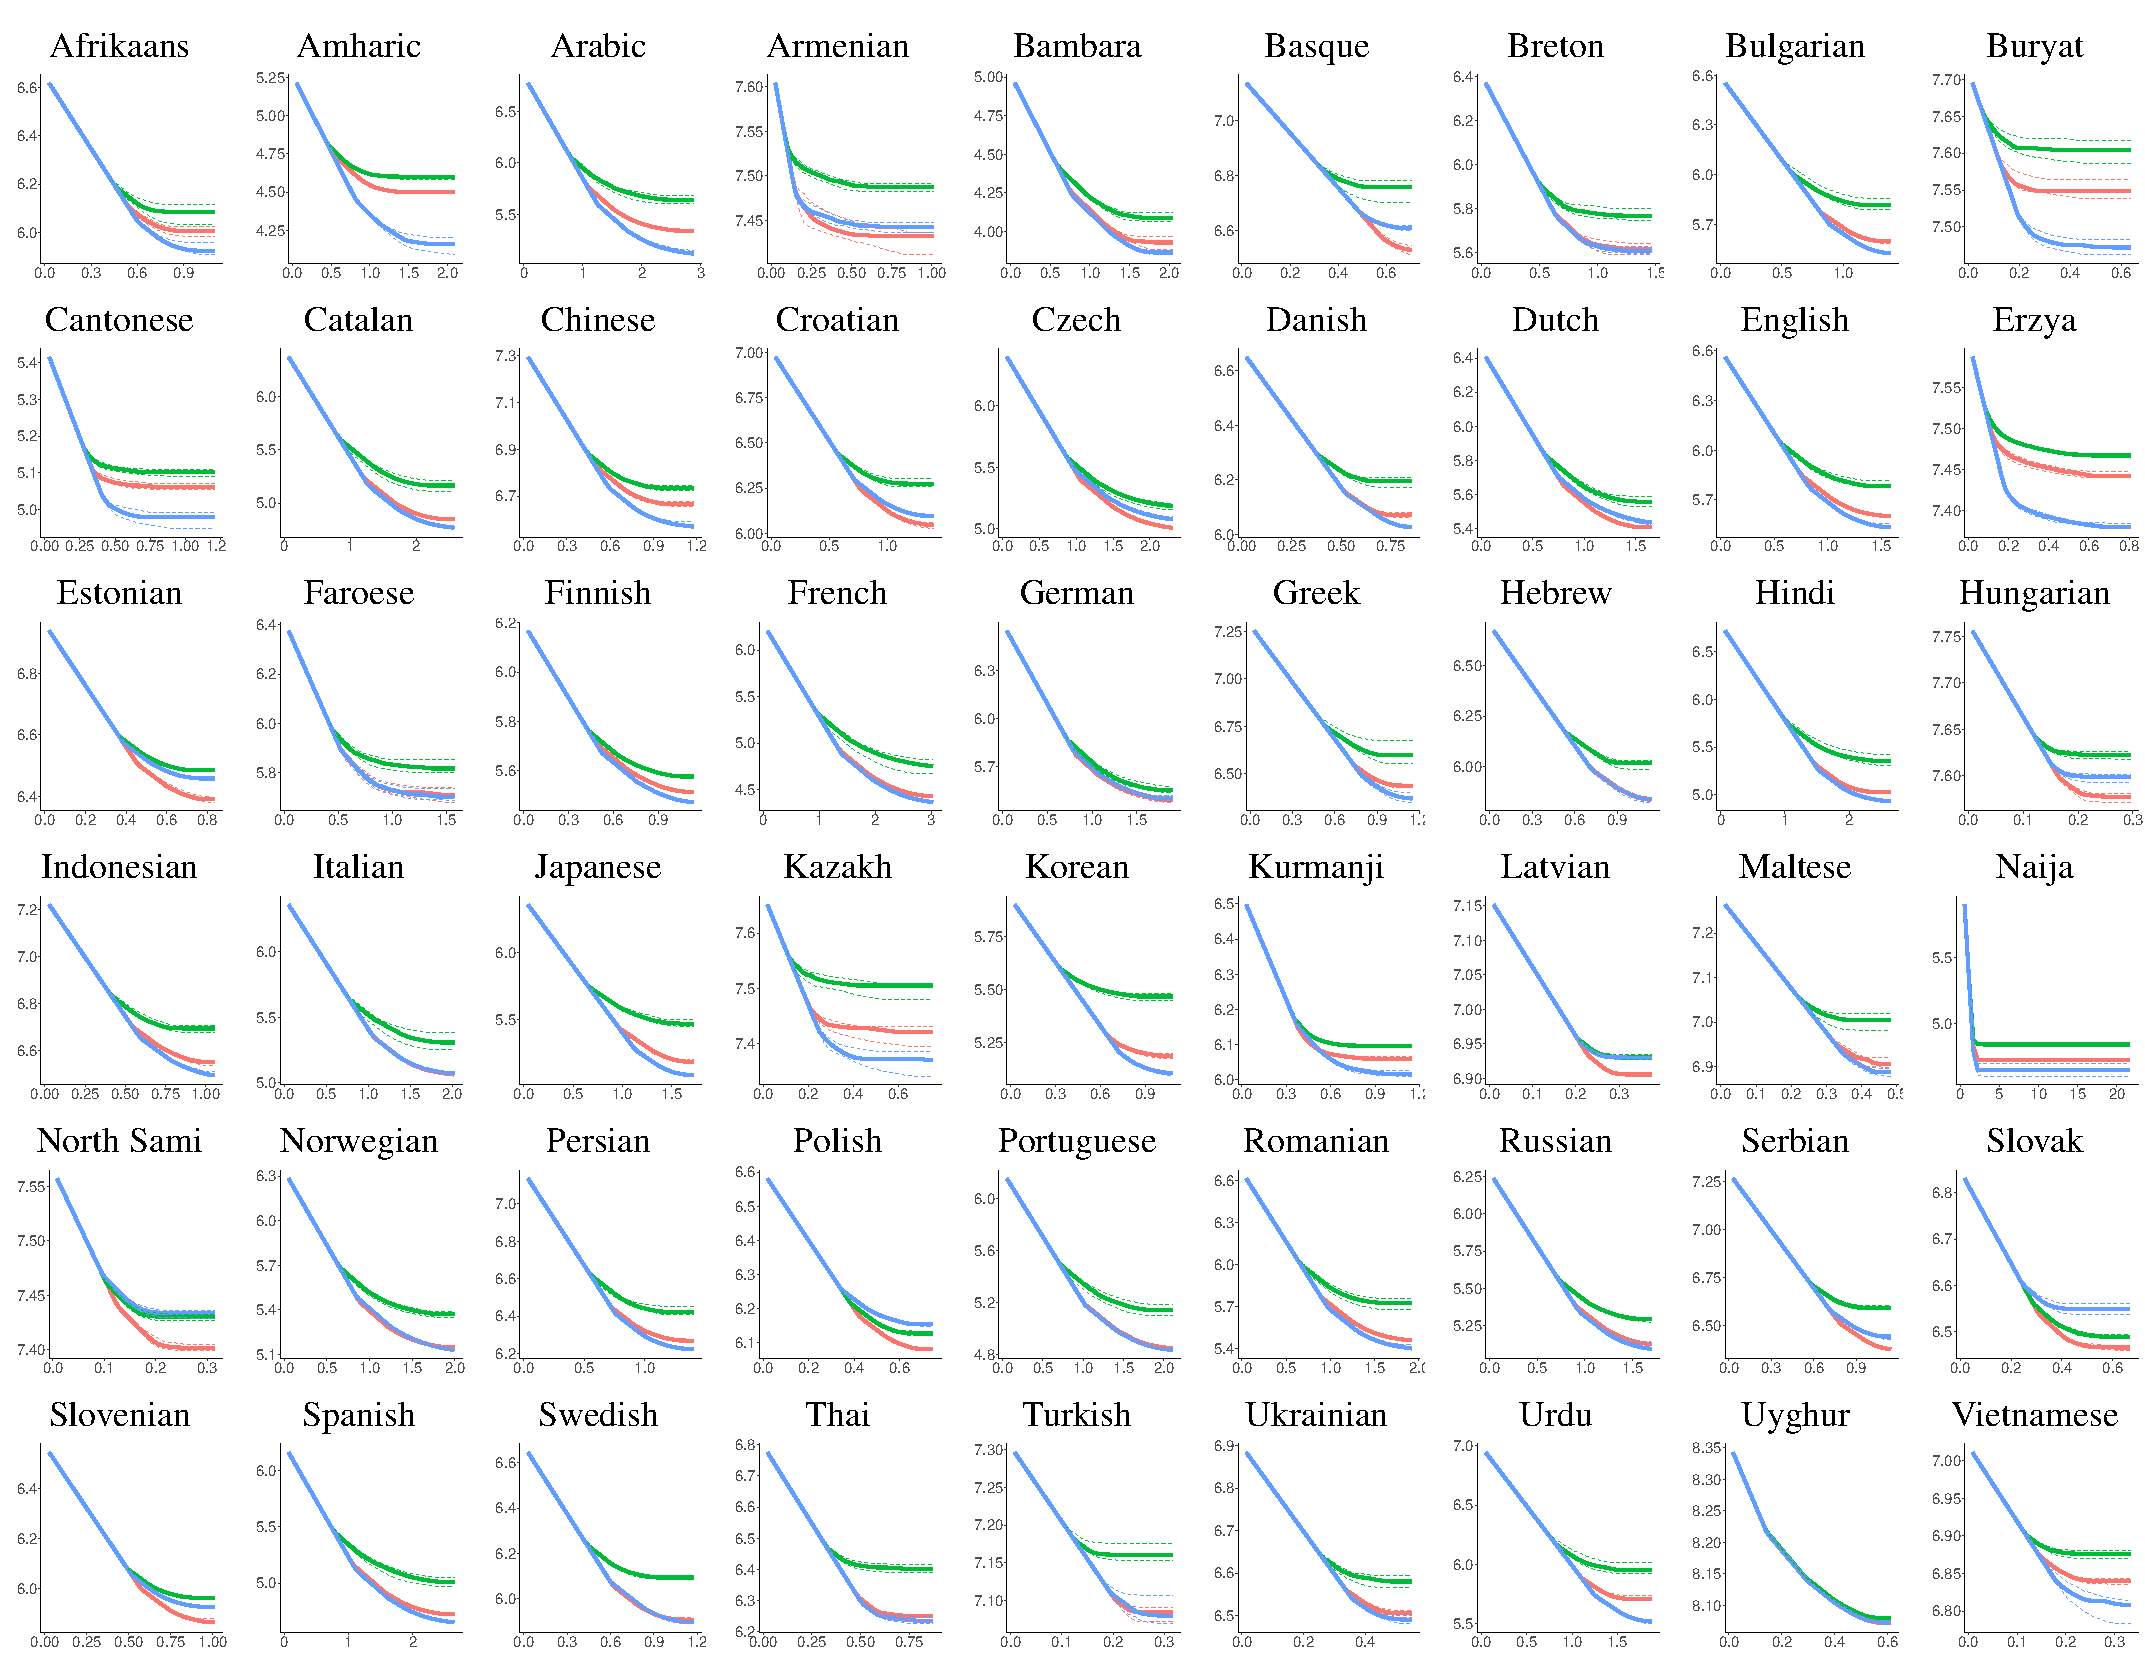
\includegraphics[width=\textwidth]{results-table-mle.pdf}
\end{center}
	\caption{Median surprisal (y-axis) at given memory level (x-axis), for real orders (blue) and random baseline grammars (red). We provide 95\% confidence bands. These are computed over different runs of the estimation algorithm for the real orders, and over different runs \emph{and} different grammars for the baseline grammars. \mhahn{make axis numbers readable}\jd{what are the green lines?}}\label{fig:median-table}
\end{figure}



\begin{figure}
	\begin{center}
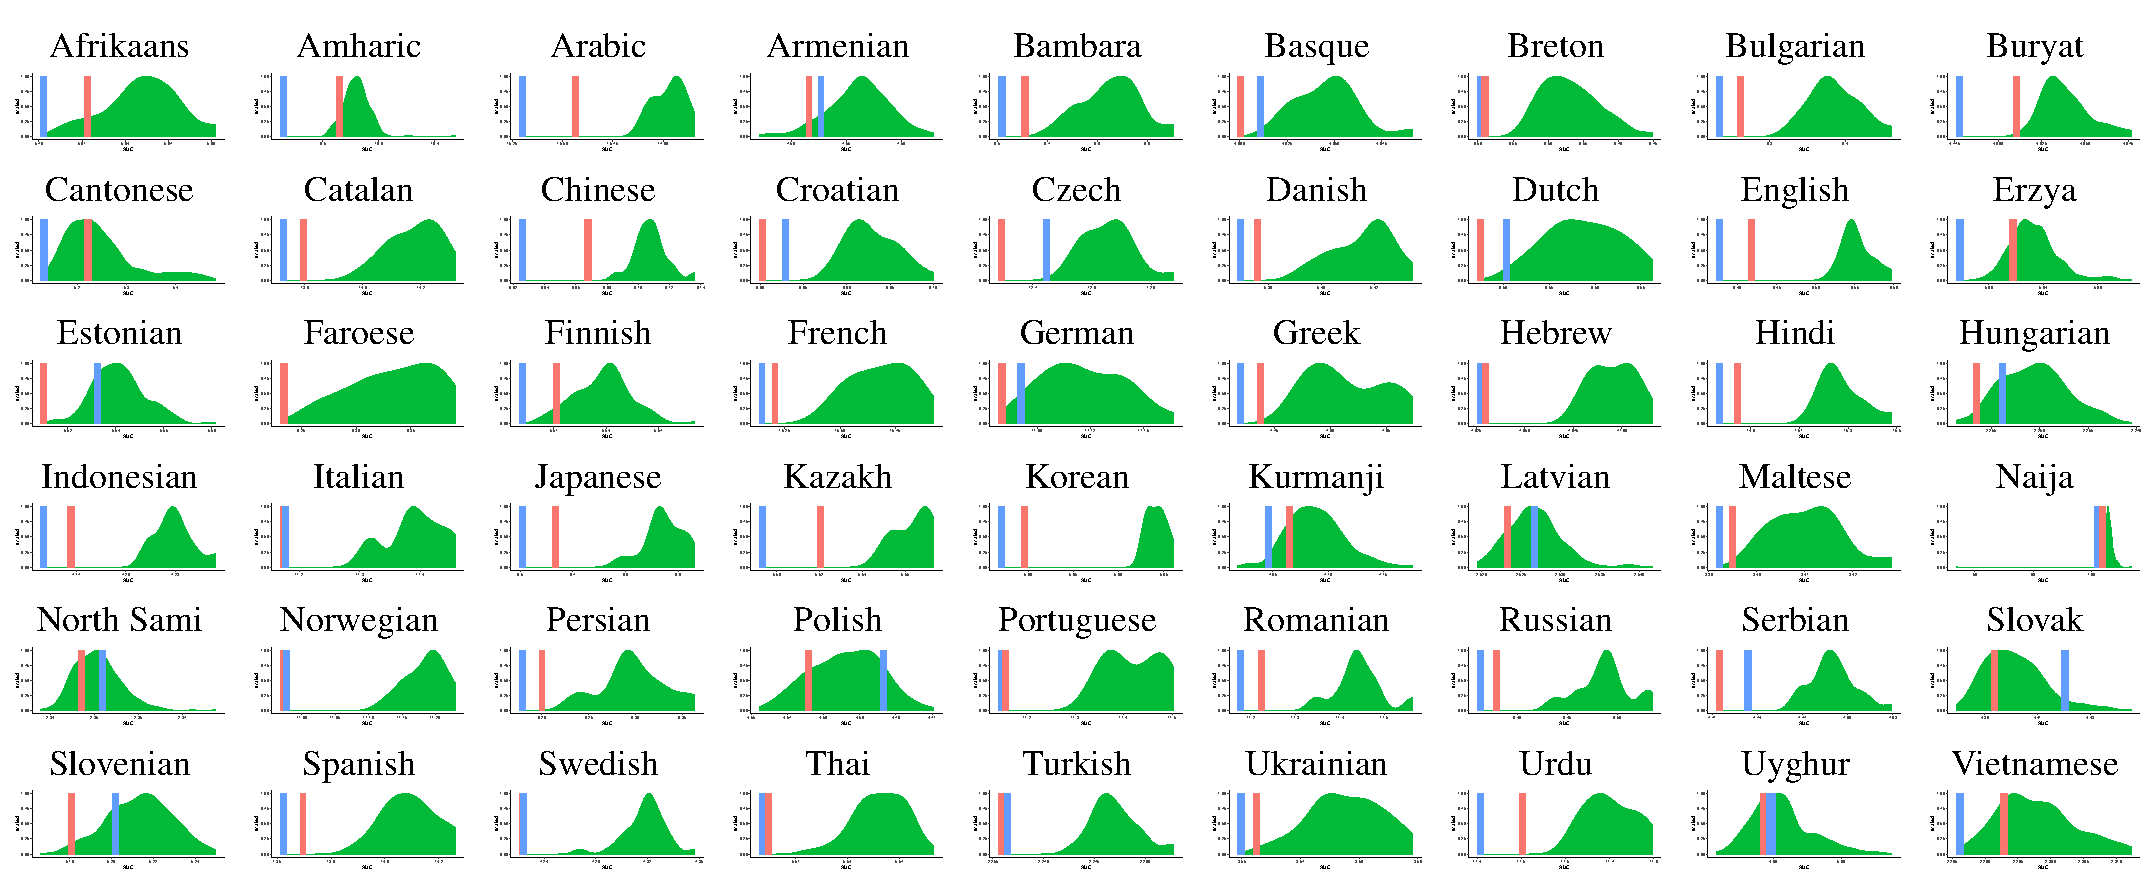
\includegraphics[width=\textwidth]{auc-table_MLE.pdf}
\end{center}
\caption{Histograms for the Area under the Curve (AUC) for the memory--surprisal tradeoffs for real (\mhahn{TODO color}) and random baseline (\mhahn{red}) orders, and for orders according to extracted grammars (\mhahn{TODO color}).
Compare Figure~\ref{fig:auc}. \mhahn{TODO make colors consistent with previous figure}
}\label{fig:auc-mle}
\end{figure}





%\begin{figure}
%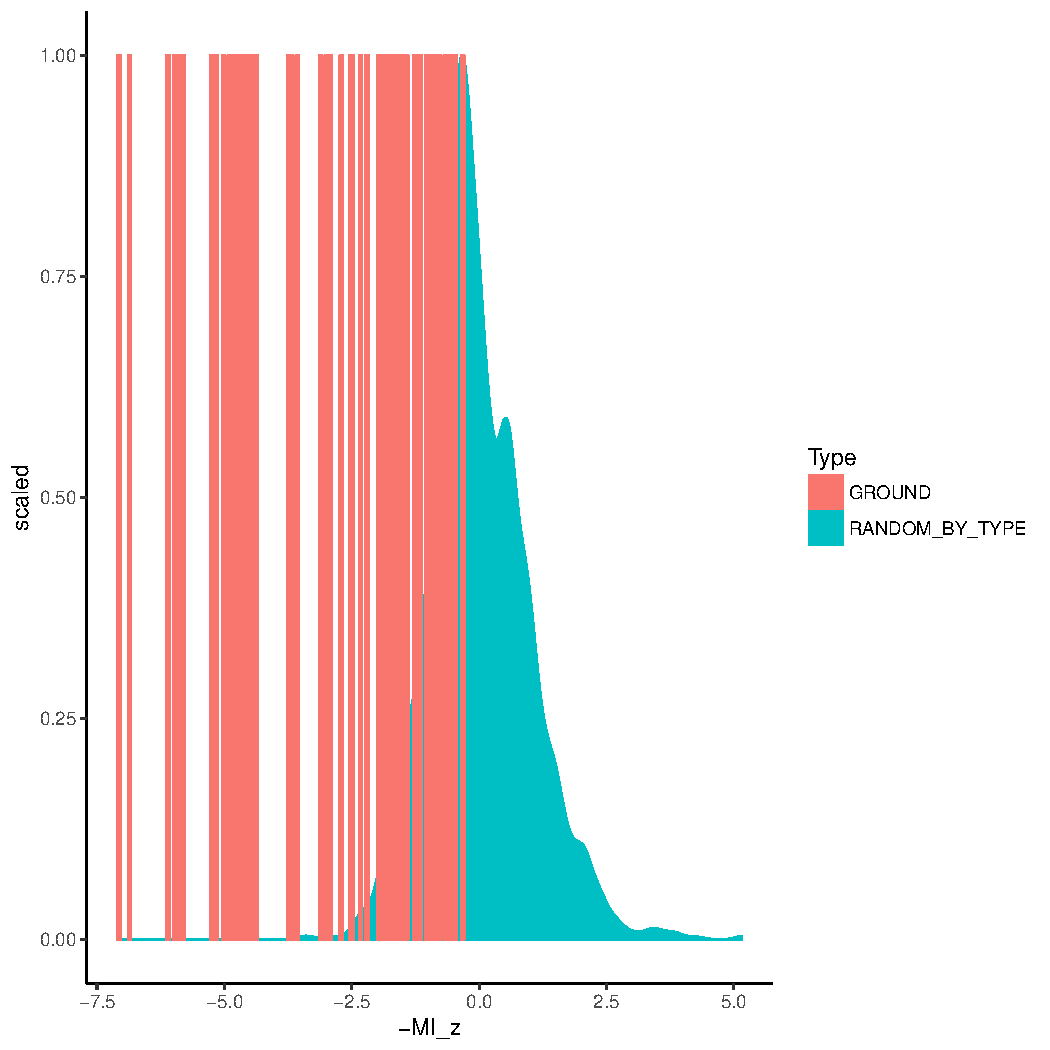
\includegraphics[width=0.5\textwidth]{figures/full-GROUND-listener-surprisal-memory-HIST_z_byMem_onlyWordForms_boundedVocab.pdf}
%	\caption{Histogram}\label{fig:hist-real}
%\end{figure}

\subsubsection{Taking Information Structure into Account}\label{sec:czech}

Languages with flexible word order often show a strong influence of information structure on word order \citep{givon1988pragmatics,jacobs1988probleme,neeleman2016word}.
Due to the difficulty of annotating information structure, only relatively few datasets have annotations for information structure, and even fewer datasets have both syntactic and information structure annotation.
We draw on the Prague Dependency Treebank of Czech \citep{bohmova2003prague,mikulova2006annotation}, which has both types of annotation.
Czech is a language with relatively high degree of word order freedom, which is generally thought to be strongly impacted by information structure \citep{firbas1966defining,firbas1974aspects}.

About one third of the Prague Dependency Treebank has annotation for topic-focus articulation \citep{mikulova2006annotation}.
Constituents are annotated for contrastiveness and for contextual boundedness, i.e., givenness.
Contextually bound expressions are presumed as given in context so that their referent is uniquely determined by the context; contextually bound expressions are contrastive if they choose from a contextually given set of alternatives \citep[Section 10.2]{mikulova2006annotation}.
Three labels are used:
``c'' for contrastive and contextually bound, ``f'' for contextually non-bound, ``t'' for non-contrastive contextually bound.
These labels were diagnosed based on constituent order and intonation.
Some constituents remain unmarked, the vast majority of which are function words such as adpositions, conjunctions, and auxiliaries; we introduce a label ``NA'' for these.
To define baselines, we extend the word order grammar formalism by defining separate weights for each combination of the 37 syntactic relations and these four information structure labels.

We obtained 38,727 training sentences and 5,228 dev sentences. We created 20 baseline grammars with information structure, 20 baseline grammars without it, and created 5 model runs for both real orders and the fitted grammar.

\paragraph{Results}

We show estimated tradeoffs and the distributions over AUC values in Figure~\ref{fig:median-czech-infostruc}.
As this experiment was conducted only on the subset of the Prague Dependency Treebank that has information structure annotation, the numerical values are slightly different from those in Section \ref{sec:main-experiment-results}. We compare the real orders both with the same baselines as above (red), and with the baselines taking information structure into account (green).
Baselines show a larger gap in efficiency between real and baseline grammars when the baselines condition word order on information structure.
This suggests that, among word orders that encode information structure, the real order of Czech provides a very efficient memory-surprisal tradeoff, and that the strength of optimization is underestimated when comparing against baselines that do not take information structure into account.

\begin{figure}
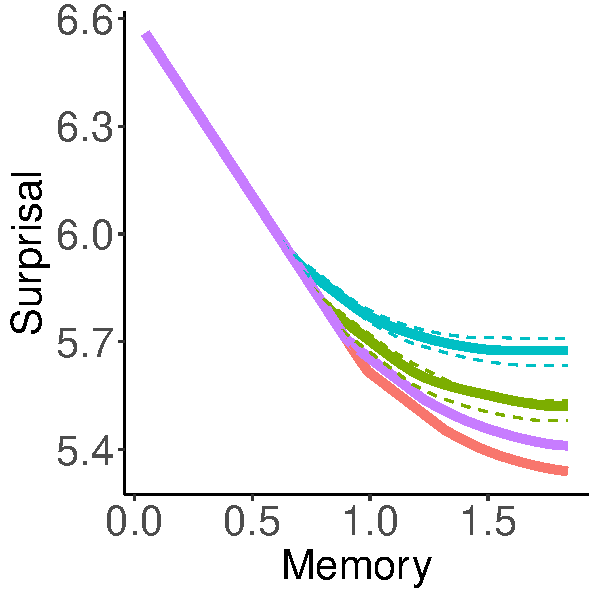
\includegraphics[width=0.5\textwidth]{figures/Czech-PDT-listener-surprisal-memory-MEDIANS_onlyWordForms_boundedVocab.pdf}
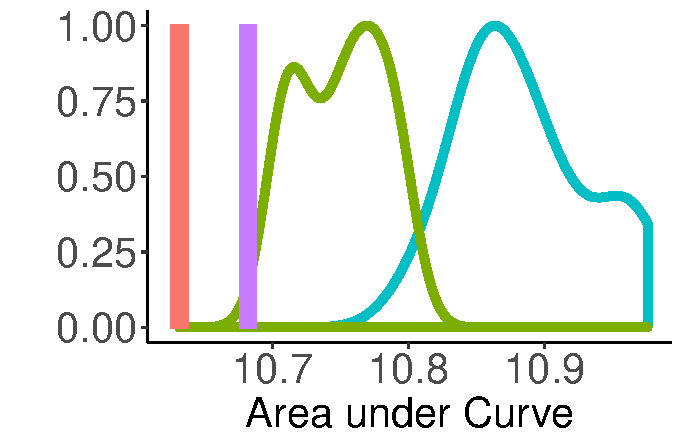
\includegraphics[width=0.5\textwidth]{figures/Czech-PDT-listener-surprisal-memory-HIST_AUC_onlyWordForms_boundedVocab_REAL-infostruc.pdf}

	\caption{Left: Memory-surprisal tradeoff Czech with information structure. Green: Baselines with information structure. Red: Baselines without information structure. Blue: Real. Right: AUC for Czech, for baselines without information structure (red) and baselines with information structure (green). Optimization of real orders is stronger when considering information structure in baselines. \mhahn{make colors compatible with previous figures}}\label{fig:median-czech-infostruc}
\end{figure}


In Figure~\ref{fig:freedom-mi-with-infostruc}, we provide a version of Figure~\ref{fig:freedom-surp} showing how the data point for Czech changes when including information structure in the  word order modeling. When modeling information structure, branching direction entropy decreases, while the surprisal difference between real and baseline orders increases.
This suggests that the weaker optimization in free word order languages observed in Study 2 might in part be because ordering grammars do not take information structure into account.
\jd{some readers will ask at this point: how does this not invalidate the whole enterprise, if adding additional information in the modeling changes the results so dramatically? and couldn't the results change in any direction? how do we know it's not a pure coincidence that it happened to go in the right direction in this case? perhaps add a sentence or two here that would assuage such a reader}
As more corpora become available, it will be important to reproduce this finding on data from further languages.
If this finding replicates, then this would mean that the impact of order freedom on the strength of optimization observed in Study 2 is an artifact of the fact that languages differ in the degree to which their word order encodes information structure, and that similar degrees of optimization might actually hold across such different languages.
	
\paragraph{Discussion}
Using data from Czech, we found that the difference between the memory-surprisal tradeoffs of real and baseline orders increases if we choose baseline orderings that encode information structure, as real orders do.
We hypothesize that this in part explains why the strength of memory efficiency optimization in Section~\ref{sec:main-experiment-results} is negatively correlated with the degree of word order freedom:
Languages with flexible word order typically encode information structure in word order, which increases average surprisal.
This does not mean that conditioning word order on information structure makes language less efficient in general.
Rather, encoding information structure in word order may increase the information content transmitted to the listener, which may in turn balance an increase in surprisal processing effort \citep{hahn2020universals}.
Due to the difficulty and cost of annotating information structure, we could only evaluate this hypothesis on data from one language.
As more annotated data becomes available, this should be replicated on data from further languages.


\subsection{Conclusion}
In this section, we tested the Efficient Tradeoff Hypothesis on dependency corpora from 54 languages, comparing observed word orders to hypothetical baseline grammars.
We found that, in 50 out of 54 languages, real orders provide more efficient memory-surprisal tradeoffs than most baseline grammars.
This suggests that, across languages, word order favors information locality more strongly than most possible alternative orders.

We also found that the degree of optimization was weaker in languages with high degrees of word order freedom.
Using data from Czech that is annotated for both syntax and information structure, we provided evidence that this dependence on word order freedom is an artifact of the fact that languages with flexible word order tend to encode information structure in word order.
%We conducted two control studies to account for word order freedom:
%First, we compared the orders of real languages with baselines in a single formalism
%\mhahn{TODO}

Taken together, Studies 1 and 2 suggest that crosslinguistic word orders are in part impacted by a pressure towards efficient memory--surprisal tradeoffs, and thus information locality.
To provide evidence that the Efficient Tradeoff Hypothesis holds at different levels of representation, we will consider morpheme order in Study 3.



	%
%\begin{figure}
%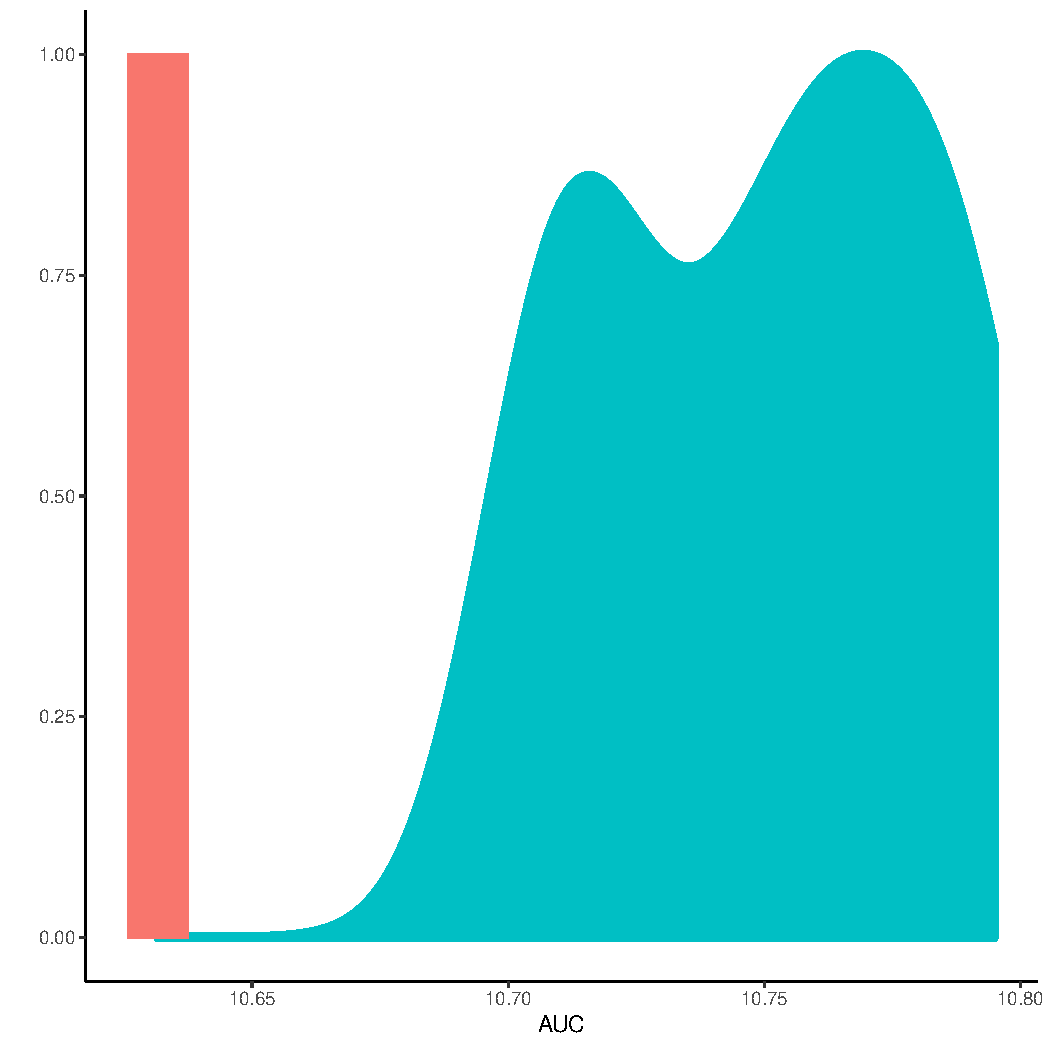
\includegraphics[width=0.5\textwidth]{figures/Czech-PDT-listener-surprisal-memory-HIST_AUC_onlyWordForms_boundedVocab_REAL-infostruc_GROUND.pdf}
%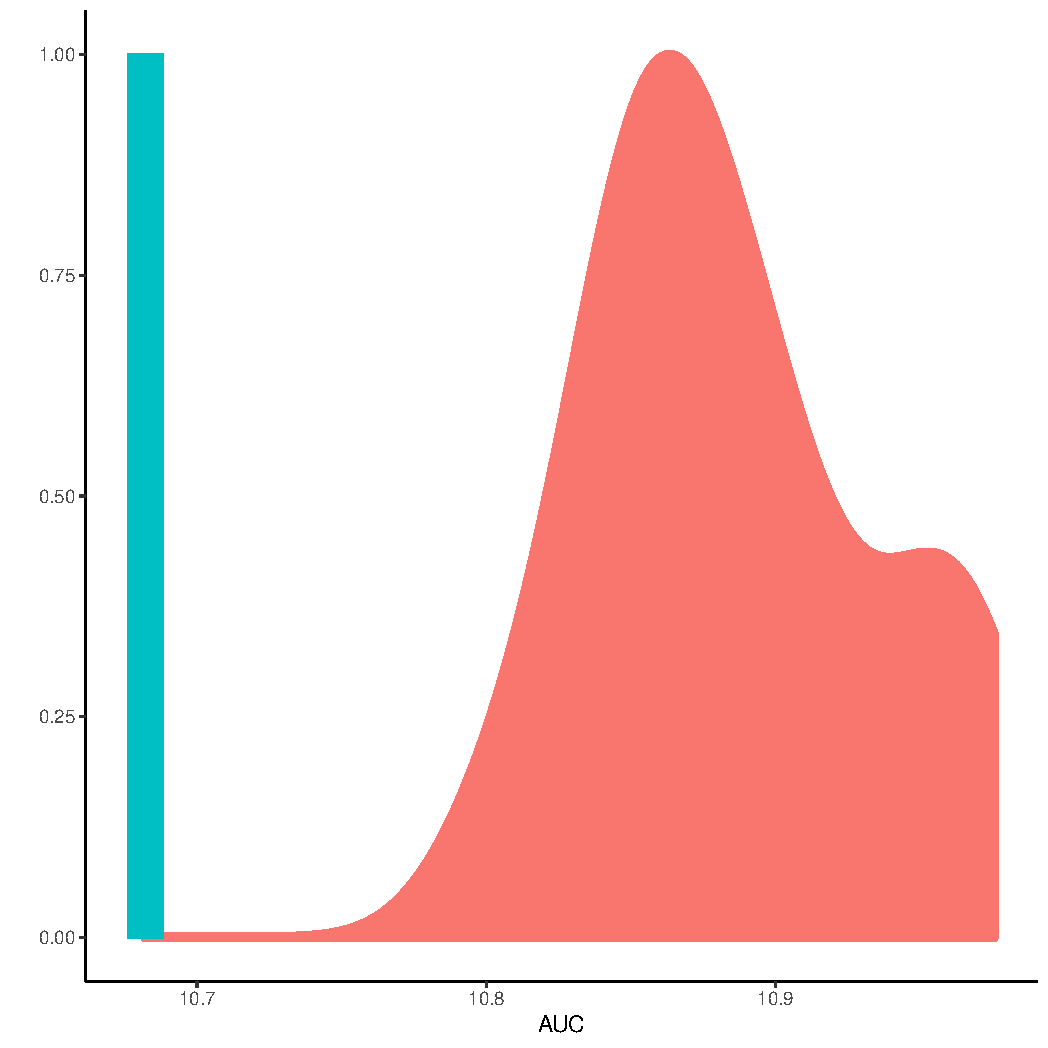
\includegraphics[width=0.5\textwidth]{figures/Czech-PDT-listener-surprisal-memory-HIST_AUC_onlyWordForms_boundedVocab_REAL-infostruc_REAL.pdf}

%	\caption{\mhahn{TODO}}\label{fig:median-czech-infostruc}
%\end{figure}





\begin{figure}
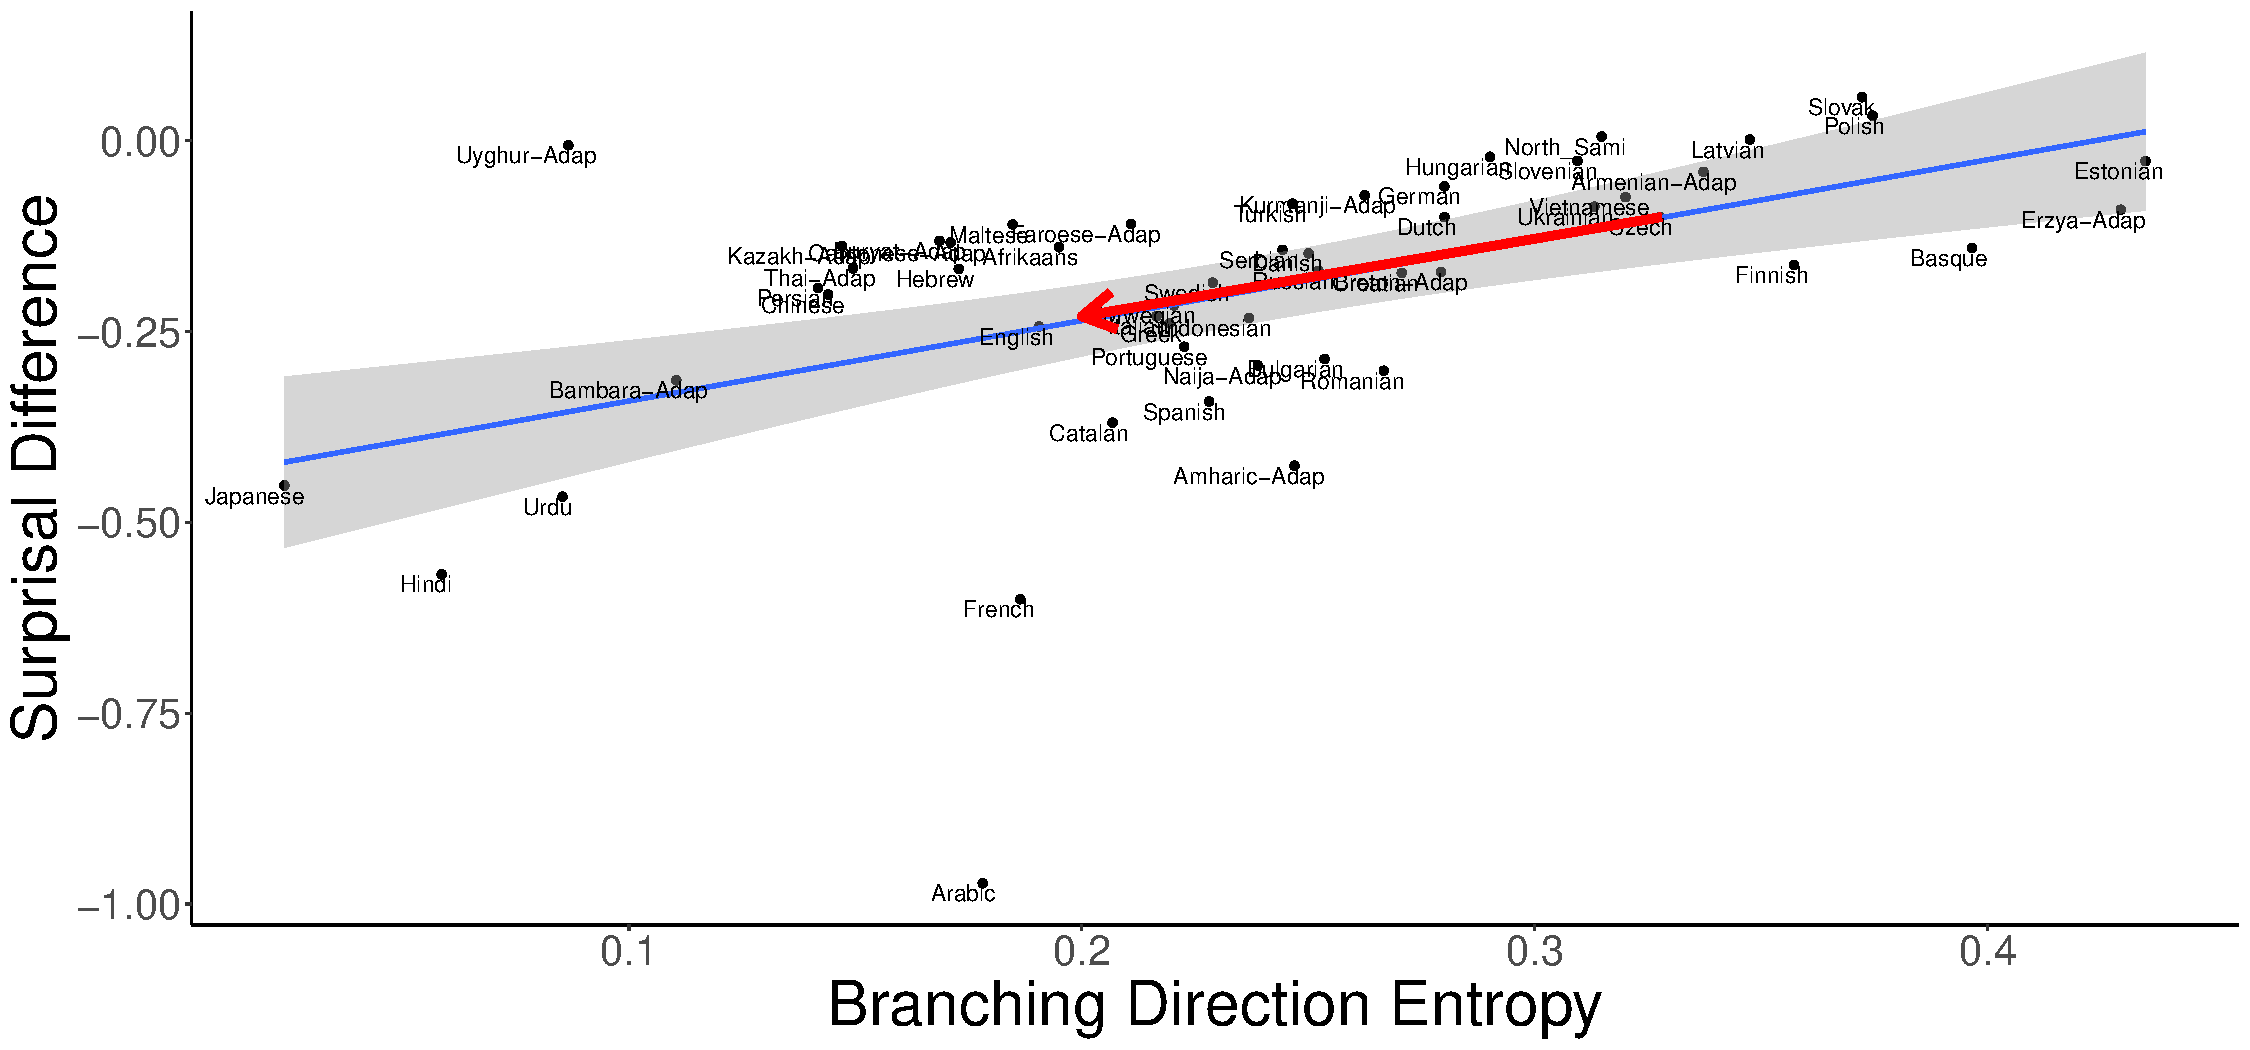
\includegraphics[width=0.9\textwidth]{figures/surprisal-branching-entropy-REAL-infostruc-invert.pdf}
	\caption{Order Freedom vs Difference in Surprisal at maximal memory (compare Figure~\ref{fig:freedom-surp}). The arrow indicates how the data point for Czech would move when modeling word order including information structure.
	When modeling information structure, branching direction entropy decreases, while the surprisal difference between real and baseline orders increases.
	This suggests that the weaker optimization in free word order languages observed in Experiment 2 might in part be because ordering grammars did not take information structure into account.\jd{this is neat, but instead of copying the whole figure, can this be integrated into the previous version of the fig?}
	}\label{fig:freedom-mi-with-infostruc}
\end{figure}




%
%\subsection{Discussion: Alternative Models}
%In view of the NLP literature, the following are the main other options that exist for estimating mutual information and probabilities in sequences:
%
%A traditional model uses n-gram models. A challenge of n-gram models is that they do not express any morphosyntactic generalizations. Furthermore, standard n-gram models do not express any generalizations about pairs of words that are not adjacent -- e.g., encoding a generalization about morphological agreement between two words is hard for such a model to capture if the two words are not always adjacent. Both the small scale of available corpora in many languages and free word order in many languages with rich morphology thus seem to make such models unattractive.
%We evaluate our hypothesis using n-gram models in SI Section X, confirming the conclusions obtained from neural models.
%
%A second option is to construct a statistical grammar, such as PCFG.
%The challenge is to encode statistical morphosyntactic generalizations, and to decide which independence assumptions to put into the model.
%One can either decide on a language-specific basis which generalizations to put in (laborious and might introduce bias), or choose a general model family that is rich enough to learn generalizations.
%The second option will make this a machine learning model that, for our purposes, does not seem to be superior to a recurrent neural network.
%



%\subsection{Data}
%\subsection{Setup}
%The recurrent neural network architecture has a range of adjustable parameters such as the number of neurons.
%For each language, we used Bayesian optimization using the Expected Improvement acquisition function (CITE) \citep{snoek-practical-2012} to find a good setting of the hyperparameters, taking average surprisal on random grammars as the objective.
%This biases the hyperparameters towards favoring counterfactual grammars.

%\subsection{Setup}




%\paragraph{Data}
%Given a sequence of input words $w_1, ..., w_n \in V$, the model 
%%
%\textbf{TODO I'm describing this in a lot of detail. Alternatively, we can say this is a standard NLP method and refer to the NLP literature for the definition.}
%The first component of such a model is an \emph{embedding matrix} $W_{emb} \in \mathbb{R}^{|V| \times d_{emb}}$, where the \emph{vocabulary} $\mathcal{V}$ is a set, containing the words that occur in the corpus, and $d_{emb} \in \mathbb{N}$ is a fixed parameter.
%This matrix assigns a $d_{emb}$-dimensional vector to each word occurring in the corpus.
%The second component is an LSTM cell $f_{LSTM}$, a nonlinear transformation mapping an \emph{input} vector $x_{i} \in \mathbb{R}^{d_{emb}}$ a \emph{hidden state} $h_i \in \mathbb{R}^{d_{LSTM}}$ and a \emph{cell state} $c_i \in \mathbb{R}^{d_{LSTM}}$ to a new pair of hidden state and cell states $h_{i+1}, c_{i+1} \in \mathbb{R}^{d_{LSTM}}$.
%The LSTM cell $f_{LSTM}$ is parameterized by a matrix of numerical parameters $W_{LSTM}$.
%
%%Such networks estimate the probability of a word in context as follows.
%Given a sequence of input words $w_1, ..., w_n \in V$, the model first retrieves fixed-dimensionality vector representations $x_1, ..., x_n$, where $x_i$ is the row of $W_{emb}$ corresponding to the word $w_i$.
%It then computes a sequence of hidden and cell states by the following recurrent computation:
%\begin{align*}
%	h_1, c_1 &:= 0 \\
%	h_2, c_2 &:= f_{LSTM}(x_1, h_1, c_1) \\
%	\dots \\
%	h_{n+1}, c_{n+1} &:= f_{LSTM}(x_n, h_n, c_n) \\
%\end{align*}
%The vector $h_i$ encodes the result of reading the words $w_1, ..., w_{i-1}$.
%We will write $LSTM(w_1, ..., w_{i-1})$ for $h_i$.
%
%The third component of the recurrent language model is the matrix $W_{output} \in \mathbb{R}^{|V| \times d_{LSTM}}$.
%We obtain per-word predictions of the next word by computing
%\begin{align*}
%	s_i := W_{output} h_i \in \mathbb{R}^{|V|} \\
%	p_i := \operatorname{softmax}(s_i)\in \mathbb{R}^{|V|} 
%\end{align*}
%where the softmax transformation normalizes vectors into probability distributions as follows
%\begin{equation}
%	\operatorname{softmax}(x)_i := \frac{\exp(x_i)}{\sum_{j=1}^{|V|} \exp(x_j)}
%\end{equation}
%Finally, the probability of the word $w_n$ in the context $w_1, ..., w_{n-1}$ is computed as
%\begin{equation}
%	p_\theta(w_n|w_1...w_{n-1}) := \frac{\exp((p_n)_{w_n})}{\sum_{w \in V} \exp(x_w)}
%\end{equation}
%and thus the surprisal is estimated as
%\begin{equation}
%- \log	p_\theta(w_n|w_1...w_{n-1}) := -\log \frac{\exp((p_n)_{w_n})}{\sum_{w \in V} \exp(x_w)}
%\end{equation}
%We discuss the choice of the numerical parameters in the next section.
%



%We collected data from the actual and random orderings in proportion one to two.
%The stopping criterion will be described below.

%Due to the randomness both in the sequence of training examples and the random initialization of the network weights, the results of the parameter estimation procedure will vary when run multiple times, especially on smaller datasets.
%Informally, due to the finiteness of the dataset, multiple parameter settings are compatible with the available training data.
%Consequently, memory-surprisal tradeoffs estimated on held-out sets will also show some variation.
%Therefore, we collect multiple samples for the actual orderings to control for variation due to the random initialization of the neural network.


%We chose these thresholds based on preliminary simulations which had suggested that these widths were achievable at acceptable computational cost.

%- at least 30 samples from both baseline and real
%
%- for the language-level tradeoff curve, either the fraction is zero or the bootstrapped CI has width $\leq 0.2$.



%
%(1) is bigram MI always greater in real languages?
%
%(2) is the tradeoff curve always lower than for deterministic simple grammar? for deterministic complex grammars? for stochastic simple/complex grammars?




%Training progresses in a series of parameter update steps, constructing updated parameters $\theta_0, \theta_1, \theta_2, \dots$.
%In the $n$-th update step, we first randomly select a word sequence $w_1 ... w_T$ from the training corpus, and use the LSTM using the current parameter setting $\theta_n$ to compute the per-word surprisals.
%We then update the parameter vector:
%\mhahn{maybe better to just say we use SGD}
%\begin{equation}\label{eq:train}
%	\theta_{n+1} := \theta_n + \alpha \partial_\theta \left(\sum_{i=1}^T \log p_\theta(w_i|w_1...w_{i-1})\right)
%\end{equation}
%where $\alpha \in \mathbb{R}_+$ is the \emph{learning rate}.



%We parameterized probabilistic ordering grammars as follows.
%For each relation type $\tau$, we introduce a \emph{direction parameter} $a_\tau \in [0,1]$ and a \emph{distance parameter} $b_\tau \in \mathbb{R}$.
%Each dependent is ordered on the left of its head with probability $a_\tau$ and to the right with probability $1-a_\tau$. 
%Then for each set of co-dependents $\{s_1, \dots , s_n\}$ placed on one side of a head, their order outward from the head is determined by iteratively sampling from the distribution $\operatorname{softmax}(b_{\tau_1}, \dots, b_{\tau_n})$ (\cite{goodfellow2016deep}, p. 184) without replacement. 
%Given a dependency tree, a probabilistic ordering grammar assigns a probability distribution over the possible projective linearizations of that tree.
%We use gradient descent to find parameters $a_\tau, b_\tau$ so as to maximize the overall likelihood of the orders in the actual corpus.
%We convert probabilistic ordering grammars into ordinary ordering grammars by the following method.
%Let $A_-$ be those relations $\tau$ where $a_\tau > 0.5$, similarly for $A_+$ those here $a_\tau \geq 0.5$.
%Then we order all relations in $A_-$ by $b_\tau$ in \emph{decreasing} order, and those in $A_+$ by $b_\tau$ in \emph{increasing} order.
%Then ordering a tree following the converted version is equivalent to greedily choosing the highest-probability linearization for the dependents of each head in a tree.
%We choose this method since maximum-likelihood grammars can be constructed with simple gradient descent.
%Another option would be to use some kind of discrete optimization method to approximate the original orders without a probabilistic method.
%However, discrete optimization is computationally challenging.


%Everything else is identical to Experiment 2.




%We test this hypothesis by comparing baseline languages to \emph{fixed-order} versions of the real languages.
%This enables us to tease apart the impact of the languages' word order rules from the impact of word order freedom.

%\mhahn{clean up text a bit}

%Above, we found that the majority of languages exhibit more favorable memory--surprisal trade-offs than counterfactual baselines based on random word order grammars. We also found that the strength of the difference between the real and baseline languages varies from language to language. Furthermore, we found that the magnitude of the difference is larger for languages with a higher degree of word order flexibility.




% Two issues: Confound because of restrictive formalism. 
% Association of efficiency and word order: By including information structure, we make the baselines worse
% Different orders based on info structure -> higher entropy when you don't have info structure

% Two controls:
% 1. Fixed-order baseline
% 2. Include info structure in the baseline, so that the baseline gets higher-entropy




